\documentclass{minimal}
\usepackage{graphicx,color}
\usepackage[utf8]{inputenc}
\usepackage[papersize={418.00bp,314.00bp},text={418.00bp,314.00bp}]{geometry}
\begin{document}
\centering
% Title: gl2ps_renderer figure
% Creator: GL2PS 1.4.2, (C) 1999-2020 C. Geuzaine
% For: Octave
% CreationDate: Thu Apr 08 16:18:14 2021
\setlength{\unitlength}{1pt}
\begin{picture}(0,0)
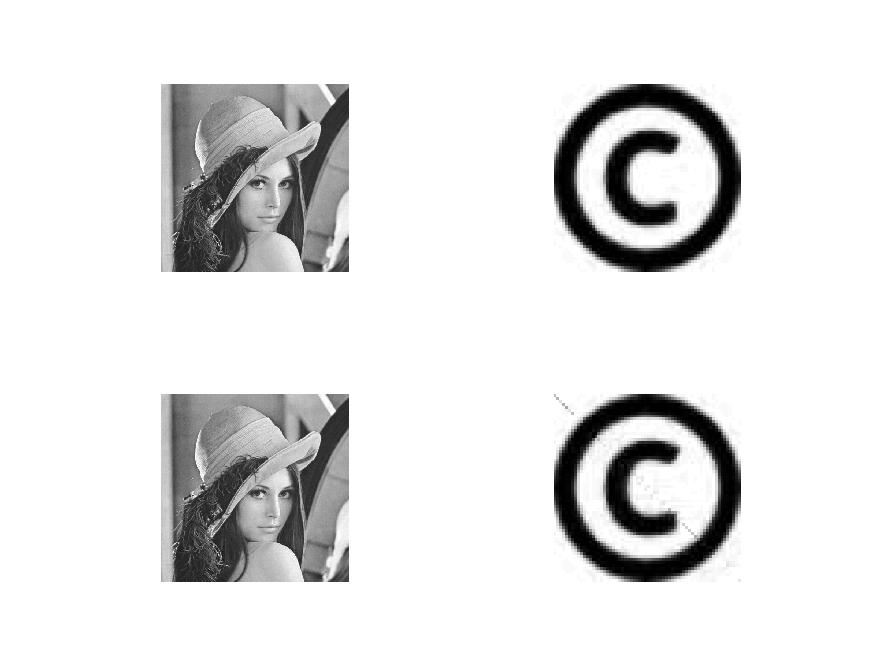
\includegraphics[scale=1]{p2_p1_plot-inc}
\end{picture}%
\begin{picture}(418,314)(0,0)
\fontsize{11}{0}\selectfont\put(122.552,283.531){\makebox(0,0)[b]{\textcolor[rgb]{0,0,0}{{Imagen original}}}}
\fontsize{11}{0}\selectfont\put(310.829,283.531){\makebox(0,0)[b]{\textcolor[rgb]{0,0,0}{{Marca de agua}}}}
\fontsize{11}{0}\selectfont\put(122.552,134.772){\makebox(0,0)[b]{\textcolor[rgb]{0,0,0}{{Imagen con la marca de agua incrustada}}}}
\fontsize{11}{0}\selectfont\put(310.829,134.772){\makebox(0,0)[b]{\textcolor[rgb]{0,0,0}{{Marca de agua extraida}}}}
\end{picture}
\end{document}
